%----------------------------------------------------------------------------------------
%    PACKAGES AND THEMES
%----------------------------------------------------------------------------------------

\documentclass[aspectratio=169,xcolor=dvipsnames]{beamer}
\usetheme{SimplePlus}
\usepackage{subcaption}
\usepackage{hyperref}
\hypersetup{colorlinks=true,linkcolor=.,urlcolor=blue,citecolor=blue}
\usepackage{amsmath}
\usepackage{xcolor}
\usepackage{graphicx}
\usepackage{booktabs}
\usepackage{tikz}
\usepackage{fontawesome5}

%----------------------------------------------------------------------------------------
%    TITLE PAGE
%----------------------------------------------------------------------------------------

\title{Explainable Disease Progression and\\Counterfactual Video Generation}
\subtitle{Complete State of the Art \& Research Plan}

\author{Mohamed BOUFAFA}

\institute
{
    Mitacs Globalink Research Internship 2026 \\[0.3em]
    T\'{E}LUQ University, Montreal, Canada \\[0.5em]
    \textbf{Supervisors:} \\
    Dr.\ Belkacem Chikhaoui (T\'{E}LUQ) \\
    Dr.\ Belkacem Khaldi (Algeria)
}
\date{April 2026 -- August 2026}

%----------------------------------------------------------------------------------------
%    PRESENTATION SLIDES
%----------------------------------------------------------------------------------------

\begin{document}

% ============================================================================
% SLIDE 1: Title
% ============================================================================
\begin{frame}
    \titlepage
\end{frame}

% ============================================================================
% SLIDE 2: Presentation Roadmap
% ============================================================================
\begin{frame}{Presentation Roadmap}
    \begin{columns}[t]
        \begin{column}{0.48\textwidth}
            \begin{block}{\textbf{Part I: Project Overview}}
                \begin{itemize}
                    \item Problem \& research gap
                    \item Five research objectives
                    \item Full pipeline at a glance
                \end{itemize}
            \end{block}

            \vspace{0.3em}

            \begin{block}{\textbf{Part II: Datasets}}
                \begin{itemize}
                    \item Yale -- primary training data
                    \item Cyprus -- validation data
                    \item Comparison \& usage strategy
                \end{itemize}
            \end{block}
        \end{column}

        \begin{column}{0.48\textwidth}
            \begin{block}{\textbf{Part III: State of the Art (15 Papers)}}
                \begin{itemize}
                    \item Phase~1: Preprocessing \& harmonization
                    \item Phase~2--3: ViT representations
                    \item Phase~4: LLM integration
                    \item Phase~5: Video generation
                \end{itemize}
            \end{block}

            \vspace{0.3em}
        \end{column}
    \end{columns}
\end{frame}

% ============================================================================
% TRANSITION: PART I
% ============================================================================
\begin{frame}[plain]
    \centering
    \vfill
    \begin{beamercolorbox}[center,shadow=true,rounded=true]{title}
        \usebeamerfont{title}
        \textbf{Part I: Project Overview}\\
        \vspace{0.5em}
        \large Problem $\to$ Objectives $\to$ Pipeline
    \end{beamercolorbox}
    \vfill
\end{frame}

% ============================================================================
% SLIDE 3: The Problem
% ============================================================================
\begin{frame}{The Problem: Static AI in a Progressive Disease}
    \begin{columns}
        \begin{column}{0.48\textwidth}
            \begin{block}{Current State of Medical AI}
                \begin{itemize}
                    \item AI segments tumors (Dice $\approx$ 0.85--0.90)
                    \item AI generates text reports
                    \item AI produces synthetic images
                \end{itemize}
            \end{block}

            \vspace{0.3em}

            \begin{alertblock}{Three Critical Gaps}
                \begin{enumerate}
                    \item \textbf{Static:} Single time-point only
                    \item \textbf{Black-box:} No plain-language reasoning
                    \item \textbf{No what-if:} Cannot simulate treatment scenarios
                \end{enumerate}
            \end{alertblock}
        \end{column}

        \begin{column}{0.48\textwidth}
            \begin{block}{What Clinicians Need}
                \begin{itemize}
                    \item Track tumor changes \textbf{over time}
                    \item Transparent reasoning (``\textit{why}'')
                    \item Visualize future progression
                    \item Compare treatment outcomes
                \end{itemize}
            \end{block}

            \vspace{0.3em}

            \begin{exampleblock}{Our Goal}
                Build an AI that \textbf{sees} (ViT), \textbf{explains} (LLM), and \textbf{imagines the future} (Video Diffusion) from longitudinal cancer scans.
            \end{exampleblock}
        \end{column}
    \end{columns}
\end{frame}

% ============================================================================
% SLIDE 4: Research Objectives
% ============================================================================
\begin{frame}{Five Research Objectives}
    \begin{columns}
        \begin{column}{0.55\textwidth}
            \begin{block}{\faIcon{bullseye} Objectives (from project proposal)}
                \small
                \begin{enumerate}
                    \item \textbf{Obj\,1 -- Data Pipeline:} Preprocess \& organize longitudinal cancer imaging data

                    \vspace{0.2em}
                    \item \textbf{Obj\,2 -- ViT Representations:} Extract temporal tumor embeddings with Vision Transformers

                    \vspace{0.2em}
                    \item \textbf{Obj\,3 -- LLM Integration:} Generate explainable clinical narratives from visual features

                    \vspace{0.2em}
                    \item \textbf{Obj\,4 -- Video Generation:} Produce counterfactual progression videos via diffusion

                    \vspace{0.2em}
                    \item \textbf{Obj\,5 -- Evaluation:} Validate with clinical metrics \& expert assessment
                \end{enumerate}
            \end{block}
        \end{column}

        \begin{column}{0.42\textwidth}
            \vspace{0.3em}

            \begin{exampleblock}{\small Literature Reviewed}
                \small \textbf{15 core papers} covering every phase.\\
                Each paper mentioned once, at the step it serves.
            \end{exampleblock}
        \end{column}
    \end{columns}
\end{frame}

% ============================================================================
% SLIDE 5: Full Pipeline at a Glance
% ============================================================================
\begin{frame}{Complete Pipeline at a Glance}
    \begin{center}
        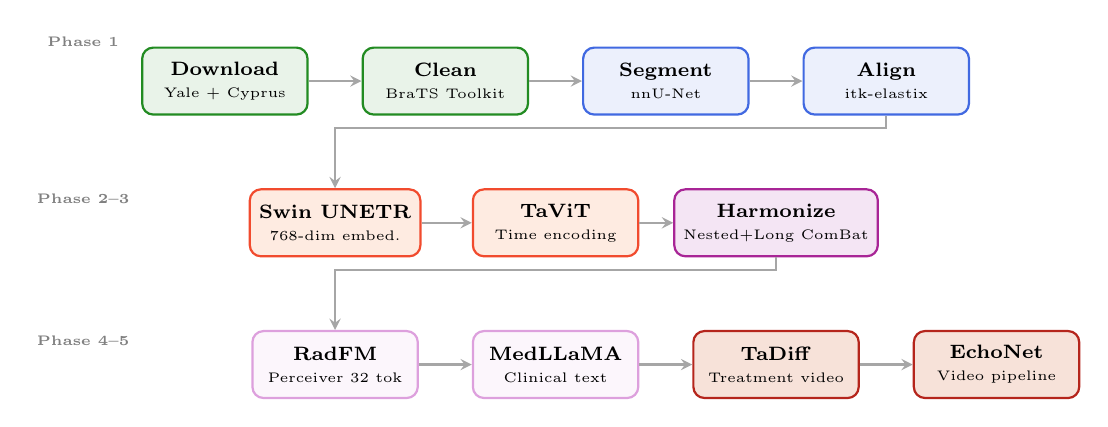
\begin{tikzpicture}[
            box/.style={rectangle, draw=#1, fill=#1!10, thick, minimum height=0.85cm, minimum width=2.1cm, align=center, rounded corners, font=\scriptsize},
            arr/.style={->, thick, >=stealth, color=gray!70},
            lbl/.style={font=\tiny\bfseries, color=gray}
        ]

        % Phase 1 row
        \node[lbl] at (-1.8,0.5) {Phase 1};
        \node[box=ForestGreen] (dl) at (0,0) {\textbf{Download}\\{\tiny Yale + Cyprus}};
        \node[box=ForestGreen] (clean) at (2.8,0) {\textbf{Clean}\\{\tiny BraTS Toolkit}};
        \node[box=RoyalBlue] (seg) at (5.6,0) {\textbf{Segment}\\{\tiny nnU-Net}};
        \node[box=RoyalBlue] (reg) at (8.4,0) {\textbf{Align}\\{\tiny itk-elastix}};

        \draw[arr] (dl) -- (clean);
        \draw[arr] (clean) -- (seg);
        \draw[arr] (seg) -- (reg);

        % Phase 2--3 row
        \node[lbl] at (-1.8,-1.5) {Phase 2--3};
        \node[box=RedOrange] (vit) at (1.4,-1.8) {\textbf{Swin UNETR}\\{\tiny 768-dim embed.}};
        \node[box=RedOrange] (tavit) at (4.2,-1.8) {\textbf{TaViT}\\{\tiny Time encoding}};
        \node[box=Mulberry] (harm) at (7,-1.8) {\textbf{Harmonize}\\{\tiny Nested+Long ComBat}};

        \draw[arr] (reg) -- ++(0,-0.6) -| (vit);
        \draw[arr] (vit) -- (tavit);
        \draw[arr] (tavit) -- (harm);

        % Phase 4 row
        \node[lbl] at (-1.8,-3.3) {Phase 4--5};
        \node[box=Plum] (radfm) at (1.4,-3.6) {\textbf{RadFM}\\{\tiny Perceiver 32 tok}};
        \node[box=Plum] (llm) at (4.2,-3.6) {\textbf{MedLLaMA}\\{\tiny Clinical text}};
        \node[box=BrickRed] (diff) at (7,-3.6) {\textbf{TaDiff}\\{\tiny Treatment video}};
        \node[box=BrickRed] (echo) at (9.8,-3.6) {\textbf{EchoNet}\\{\tiny Video pipeline}};

        \draw[arr] (harm) -- ++(0,-0.6) -| (radfm);
        \draw[arr] (radfm) -- (llm);
        \draw[arr] (llm) -- (diff);
        \draw[arr] (diff) -- (echo);

        \end{tikzpicture}
    \end{center}

    \vspace{0.3em}

    \begin{columns}
        \begin{column}{0.32\textwidth}
            \centering
            \textbf{Step 1:} Prepare \& Extract\\
            \small 768-dim per scan
        \end{column}
        \begin{column}{0.32\textwidth}
            \centering
            \textbf{Step 2:} Explain\\
            \small Clinical narrative
        \end{column}
        \begin{column}{0.32\textwidth}
            \centering
            \textbf{Step 3:} Generate\\
            \small Counterfactual video
        \end{column}
    \end{columns}
\end{frame}

% ============================================================================
% TRANSITION: PART II -- DATASETS
% ============================================================================
\begin{frame}[plain]
    \centering
    \vfill
    \begin{beamercolorbox}[center,shadow=true,rounded=true]{title}
        \usebeamerfont{title}
        \textbf{Part II: Datasets}\\
        \vspace{0.5em}
        \large Yale (Training) $\to$ Cyprus (Validation)
    \end{beamercolorbox}
    \vfill
\end{frame}

% ============================================================================
% SLIDE 6: Why Longitudinal Data
% ============================================================================
\begin{frame}{Why Longitudinal Data? Existing Datasets Fall Short}
    \begin{columns}
        \begin{column}{0.48\textwidth}
            \begin{alertblock}{The Project Requirement}
                \small
                Our project needs \textbf{longitudinal} imaging: the same patient scanned multiple times over months/years to model disease \textbf{progression} and \textbf{treatment response}.
            \end{alertblock}

            \vspace{0.2em}

            \begin{block}{Common Datasets Are Static}
                \small
                \begin{itemize}
                    \item \textbf{BraTS}: Single time-point per patient
                    \item \textbf{TCGA}: Mostly single snapshots
                    \item \textbf{LIDC-IDRI}: CT lung, no follow-up
                \end{itemize}
                $\Rightarrow$ None support temporal modeling!
            \end{block}
        \end{column}

        \begin{column}{0.48\textwidth}
            \begin{exampleblock}{Our Solution: Two Complementary Datasets}
                \small
                \begin{enumerate}
                    \item \textbf{Yale} (2025): Largest longitudinal brain MRI ever released -- 11,884 scans, 1,430 patients
                    \item \textbf{Cyprus PROTEAS} (2025): Small but richly labeled -- 744 scans, 40 patients with expert segmentations
                \end{enumerate}
            \end{exampleblock}

            \vspace{0.2em}

            \begin{block}{\small Strategy}
                \scriptsize
                \faIcon{check} Train on Yale (large scale)\\
                \faIcon{check} Validate on Cyprus (ground truth labels)\\
                \faIcon{check} Both FREE and PUBLIC
            \end{block}
        \end{column}
    \end{columns}
\end{frame}

% ============================================================================
% SLIDE 7: Yale Dataset
% ============================================================================
\begin{frame}{Paper~01: Yale Longitudinal Brain Metastases Dataset (2025)}
    \begin{columns}
        \begin{column}{0.52\textwidth}
            \begin{block}{Summary}
                \small
                \href{https://doi.org/10.1038/s41597-025-04360-7}{Ramakrishnan et al., \textit{Scientific Data}, 2025}\\[0.3em]
                Largest public longitudinal brain MRI dataset for brain metastases research.
            \end{block}

            \vspace{0.2em}

            \begin{block}{Key Numbers}
                \small
                \begin{tabular}{ll}
                    Patients & 1,430 \\
                    Total scans & 11,884 \\
                    Avg scans/patient & 8.3 \\
                    Time span & 2004--2023 (20 years) \\
                    Modalities & T1, T1c, T2, FLAIR \\
                    Scanners & Siemens 86\%, GE 13\% \\
                    Field strength & 3T (41\%), 1.5T (58\%) \\
                \end{tabular}
            \end{block}
        \end{column}

        \begin{column}{0.44\textwidth}
            \begin{block}{Why This Dataset}
                \small
                \begin{itemize}
                    \item First large-scale \textbf{longitudinal} public brain MRI
                    \item Avg 8.3 visits $\Rightarrow$ temporal sequences
                    \item Pre- and post-treatment scans
                    \item Clinical metadata included
                \end{itemize}
            \end{block}

            \vspace{0.1em}

            \begin{alertblock}{Challenges We Must Solve}
                \small
                $\triangle$ \textbf{No tumor labels} $\to$ generate with nnU-Net\\
                $\triangle$ \textbf{5+ batch effects} $\to$ Nested ComBat\\
                % $\triangle$ Variable quality over 20 years
            \end{alertblock}

            \begin{exampleblock}{\scriptsize \faIcon{database} Access}
                \scriptsize \href{https://www.cancerimagingarchive.net/}{TCIA} -- Free, DOI: 10.7937/3YAT-E768
            \end{exampleblock}
        \end{column}
    \end{columns}
\end{frame}

% ============================================================================
% SLIDE 8: Cyprus Dataset
% ============================================================================
\begin{frame}{Paper~02: Cyprus PROTEAS Dataset (2025)}
    \begin{columns}
        \begin{column}{0.52\textwidth}
            \begin{block}{Summary}
                \small
                \href{https://doi.org/10.5281/zenodo.17253793}{Trimithiotis et al., 2025}\\[0.3em]
                Smaller but richly annotated longitudinal brain MRI with \textbf{expert-verified tumor labels}.
            \end{block}

            \vspace{0.2em}

            \begin{block}{Key Numbers}
                \small
                \begin{tabular}{ll}
                    Patients & 40 \\
                    Total scans & 744 \\
                    Avg scans/patient & 18.6 (2$\times$ Yale!) \\
                    Labeled tumors & 65 (3 subregions) \\
                    Radiomic features & 110 pre-extracted \\
                    Primary cancer & Lung 67.5\%, Breast 32.5\% \\
                \end{tabular}
            \end{block}
        \end{column}

        \begin{column}{0.44\textwidth}
            \begin{block}{What Cyprus Adds}
                \small
                \begin{itemize}
                    \item \textbf{3-subregion segmentations:} enhancing, necrosis, edema
                    \item Expert neuroradiologist verified
                    \item Radiotherapy plans (45 RTP)
                    \item Survival data included
                \end{itemize}
            \end{block}

            \vspace{0.2em}

            \begin{alertblock}{Role: External Validation}
                \small
                Train on Yale $\to$ test on Cyprus\\
                Different hospital, country, scanners\\
                $\Rightarrow$ Proves our pipeline generalizes
            \end{alertblock}

            \begin{exampleblock}{\scriptsize \faIcon{database} Access}
                \scriptsize \href{https://zenodo.org/}{Zenodo} -- Free, open access
            \end{exampleblock}
        \end{column}
    \end{columns}
\end{frame}

% ============================================================================
% SLIDE 9: Dataset Comparison
% ============================================================================
\begin{frame}{Dataset Comparison: Yale vs.\ Cyprus}
    \begin{columns}
        \begin{column}{0.55\textwidth}
            \begin{table}
                \centering
                \footnotesize
                \begin{tabular}{lcc}
                    \toprule
                    \textbf{Feature} & \textbf{Yale} & \textbf{Cyprus} \\
                    \midrule
                    Role & Training & Validation \\
                    Patients & 1,430 & 40 \\
                    Total scans & 11,884 & 744 \\
                    Scans/patient & 8.3 & 18.6 \\
                    Tumor labels & \textcolor{red}{\faIcon{times}} & \textcolor{green}{\faIcon{check}} (expert) \\
                    Radiomic features & \textcolor{red}{\faIcon{times}} & \textcolor{green}{\faIcon{check}} (110) \\
                    Radiotherapy plans & \textcolor{red}{\faIcon{times}} & \textcolor{green}{\faIcon{check}} (45) \\
                    Survival data & \textcolor{red}{\faIcon{times}} & \textcolor{green}{\faIcon{check}} \\
                    Scanners & Siemens/GE & Philips/Siemens \\
                    Already preprocessed & \textcolor{red}{\faIcon{times}} & \textcolor{green}{\faIcon{check}} \\
                    Cost & Free & Free \\
                    \bottomrule
                \end{tabular}
            \end{table}
        \end{column}

        \begin{column}{0.42\textwidth}
            \begin{exampleblock}{Combined Usage}
                \small
                \begin{enumerate}
                    \item \textbf{Train} on Yale (1,430 patients)
                    \item \textbf{Validate segmentation} on Cyprus expert labels (65 tumors, target Dice $>0.85$)
                    \item \textbf{Test harmonization} across scanner vendors (Siemens $\leftrightarrow$ Philips)
                    \item \textbf{Validate videos} using Cyprus's denser temporal coverage (18.6 scans/patient)
                \end{enumerate}
            \end{exampleblock}

            \vspace{0.2em}

            \begin{alertblock}{\small Why Not Merge?}
                \scriptsize Cyprus is too small (40 patients) to add to training, and merging would invalidate external validation.
            \end{alertblock}
        \end{column}
    \end{columns}
\end{frame}

% ============================================================================
% TRANSITION: PART III -- STATE OF THE ART
% ============================================================================
\begin{frame}[plain]
    \centering
    \vfill
    \begin{beamercolorbox}[center,shadow=true,rounded=true]{title}
        \usebeamerfont{title}
        \textbf{Part III: State of the Art}\\
        \vspace{0.5em}
        \large 15 Papers Across All Phases
    \end{beamercolorbox}
    \vfill
\end{frame}

% ============================================================================
% SLIDE 10: Paper Map
% ============================================================================
\begin{frame}{Paper Map: 15 Papers, One Per Pipeline Step}
    \begin{table}
        \centering
        \footnotesize
        \begin{tabular}{clll}
            \toprule
            \textbf{\#} & \textbf{Paper} & \textbf{What We Take} & \textbf{Phase} \\
            \midrule
            01 & Yale Dataset (Ramakrishnan 2025) & Primary training data (11,884 scans) & 1 \\
            02 & Cyprus PROTEAS (Trimithiotis 2025) & Validation ground truth (expert labels) & 1 \\
            03 & BraTS Toolkit (Kofler 2020) & HD-BET skull stripping & 1 \\
            04 & nnU-Net (Isensee 2021) & BraTS-pretrained tumor segmentation & 1 \\
            05 & itk-elastix (Niessen 2023) & Longitudinal registration (rigid + deformable) & 1 \\
            06 & Generalized ComBat (Horng 2022) & Nested ComBat for 5+ batch effects & 3 \\
            07 & Longitudinal ComBat (Beer 2020) & Preserve within-patient trajectories & 3 \\
            08 & ComBat Guide (Fortin 2022) & Feature-space harmonization theory & 3 \\
            09 & Swin UNETR (Tang 2022) & 768-dim feature extractor & 3 \\
            10 & TaViT (Hager 2022) & Time-distance positional encoding & 3 \\
            11 & RadFM (Wu 2025) & Perceiver (32 tokens) + MedLLaMA-13B & 4 \\
            12 & MM-Embed (Lin 2025) & Contrastive embedding alignment & 4 \\
            13 & LDM (Rombach 2022) & Latent diffusion + VAE + cross-attention & 5 \\
            14 & TaDiff (Liu 2025) & Treatment-aware generation + counterfactual & 5 \\
            15 & EchoNet-Synthetic (Reynaud 2024) & Video diffusion pipeline (starting code) & 5 \\
            \bottomrule
        \end{tabular}
    \end{table}
\end{frame}

% ============================================================================
% SECTION: PHASE 1 PAPERS
% ============================================================================
\begin{frame}[plain]
    \centering
    \vfill
    \begin{beamercolorbox}[center,shadow=true,rounded=true]{title}
        \usebeamerfont{title}
        \textbf{Phase~1: Preprocessing}\\
        \vspace{0.5em}
        \large Skull Stripping $\to$ Segmentation $\to$ Registration
    \end{beamercolorbox}
    \vfill
\end{frame}

% ============================================================================
% SLIDE 11: BraTS Toolkit
% ============================================================================
\begin{frame}{Paper~03: BraTS Toolkit -- Preprocessing Pipeline (2020)}
    \begin{columns}
        \begin{column}{0.52\textwidth}
            \begin{block}{Summary}
                \small
                \href{https://doi.org/10.3389/fnins.2020.00125}{Kofler et al., \textit{Frontiers in Neuroscience}, 2020}\\[0.3em]
                Standardized preprocessing toolkit: skull stripping, normalization, and format conversion for brain tumor MRI.
            \end{block}

            \vspace{0.2em}

            \begin{block}{What It Does (One Command)}
                \small
                \begin{enumerate}
                    \item Co-register T1/T1c/T2/FLAIR \textbf{within one visit}
                    \item \textbf{HD-BET} skull stripping (AI-based)
                    \item Resample to 1\,mm$^3$ isotropic
                \end{enumerate}
                \vspace{0.2em}
                {\scriptsize Note: Yale is already NIfTI -- skip DICOM conversion}
            \end{block}
        \end{column}

        \begin{column}{0.44\textwidth}
            \begin{alertblock}{For Our Project}
                \small
                Clean all 11,884 Yale scans in one step.\\[0.3em]
                \textbf{Important:} BraTS aligns modalities \textbf{within} one visit.\\
                Cross-visit alignment requires itk-elastix (Paper~05).
            \end{alertblock}

            \vspace{0.2em}

            \begin{exampleblock}{\scriptsize \faIcon{github} Code}
                \scriptsize \href{https://github.com/neuronflow/BraTS-Toolkit}{neuronflow/BraTS-Toolkit} (Python, pip install)
            \end{exampleblock}
        \end{column}
    \end{columns}
\end{frame}

% ============================================================================
% SLIDE 12: nnU-Net
% ============================================================================
\begin{frame}{Paper~04: nnU-Net -- Tumor Segmentation (2021)}
    \begin{columns}
        \begin{column}{0.52\textwidth}
            \begin{block}{Summary}
                \small
                \href{https://doi.org/10.1038/s41592-020-01008-z}{Isensee et al., \textit{Nature Methods}, 2021}\\[0.3em]
                Self-configuring segmentation framework. Automatically adapts architecture, preprocessing, and training to any dataset.
            \end{block}

            \vspace{0.2em}

            \begin{block}{Key Results}
                \small
                \begin{itemize}
                    \item BraTS 2021: \textbf{3-region segmentation}
                        \begin{itemize}
                            \scriptsize
                            \item Enhancing Tumor: Dice 0.85
                            \item Tumor Core: Dice 0.88
                            \item Whole Tumor: Dice 0.91
                        \end{itemize}
                    \item \textbf{1st place} BraTS 2020 \& 2021
                    \item BraTS-pretrained weights available
                \end{itemize}
            \end{block}
        \end{column}

        \begin{column}{0.44\textwidth}
            \begin{alertblock}{For Our Project}
                \small
                Yale has \textbf{no tumor labels}.\\
                $\Rightarrow$ Generate \textbf{3-region masks} (enhancing, necrotic, edema) for all 11,884 scans.\\[0.3em]
                Validate on Cyprus 3-subregion expert labels (target Dice $>0.85$).
            \end{alertblock}

            \vspace{0.2em}

            \begin{block}{\small Also Serves As}
                \small CNN baseline to beat with Swin UNETR (Phase~3).
            \end{block}

            \begin{exampleblock}{\scriptsize \faIcon{github} Code}
                \scriptsize \href{https://github.com/MIC-DKFZ/nnUNet}{MIC-DKFZ/nnUNet} (PyTorch)
            \end{exampleblock}
        \end{column}
    \end{columns}
\end{frame}

% ============================================================================
% SLIDE 13: itk-elastix
% ============================================================================
\begin{frame}{Paper~05: itk-elastix -- Longitudinal Registration (2023)}
    \begin{columns}
        \begin{column}{0.52\textwidth}
            \begin{block}{Summary}
                \small
                \href{https://doi.org/10.21105/joss.05421}{Niessen et al., \textit{JOSS}, 2023}\\[0.3em]
                Python wrapper for Elastix: rigid + deformable registration for aligning brain scans \textbf{across different visits} over time.
            \end{block}

            \vspace{0.2em}

            \begin{block}{What It Does}
                \small
                \begin{enumerate}
                    \item Rigid registration (correct head position)
                    \item B-spline deformable (correct brain shift)
                    \item Produces deformation field per voxel
                \end{enumerate}
            \end{block}
        \end{column}

        \begin{column}{0.44\textwidth}
            \begin{alertblock}{For Our Project}
                \small
                Each patient has $\sim$8 visits. Align all to first visit ($T_0$) so tumor changes are spatially comparable.\\[0.3em]
                Without this, can't tell if a voxel changed because tumor grew \textit{or} head tilted differently.
            \end{alertblock}

            \vspace{0.2em}

            \begin{block}{\small Why Not FLIRE?}
                \scriptsize
                FLIRE is MATLAB-based (no Python API).\\
                itk-elastix is pip-installable + actively maintained.
            \end{block}

            \begin{exampleblock}{\scriptsize \faIcon{github} Code}
                \scriptsize \texttt{pip install itk-elastix} (Python)
            \end{exampleblock}
        \end{column}
    \end{columns}
\end{frame}

% ============================================================================
% SECTION: PHASE 3 PAPERS
% ============================================================================
\begin{frame}[plain]
    \centering
    \vfill
    \begin{beamercolorbox}[center,shadow=true,rounded=true]{title}
        \usebeamerfont{title}
        \textbf{Phase~3: Vision Transformers + Harmonization}\\
        \vspace{0.5em}
        \large Swin UNETR $\to$ TaViT $\to$ Nested + Longitudinal ComBat
    \end{beamercolorbox}
    \vfill
\end{frame}

% ============================================================================
% SLIDE 14: Swin UNETR
% ============================================================================
\begin{frame}{Paper~09: Swin UNETR -- Feature Extractor (2022)}
    \begin{columns}
        \begin{column}{0.52\textwidth}
            \begin{block}{Summary}
                \small
                \href{https://arxiv.org/abs/2201.01266}{Tang et al., CVPR 2022}\\[0.3em]
                Hierarchical Swin Transformer encoder + U-Net decoder for 3D medical image segmentation. Self-supervised pre-training on 5,050 CT scans.
            \end{block}

            \vspace{0.2em}

            \begin{block}{Key Results}
                \small
                \begin{itemize}
                    \item BraTS 2021: \textbf{3-region segmentation}
                        \begin{itemize}
                            \scriptsize
                            \item Enhancing Tumor: Dice 0.858
                            \item Tumor Core: Dice 0.885
                            \item Whole Tumor: Dice 0.926
                        \end{itemize}
                    \item \textbf{one of the top places in} BraTS 2021 challange
                    \item BraTS-pretrained weights available
                \end{itemize}
            \end{block}
        \end{column}

        \begin{column}{0.44\textwidth}
            \begin{alertblock}{For Our Project}
                \small
                \textbf{Two-step approach:}\\[0.2em]
                \scriptsize
                1. Load MONAI pre-trained weights (5,050 CT scans)\\
                2. Fine-tune on Yale brain MRI (11,884 scans)\\
                3. Use \textbf{encoder only} $\to$ 768-dim embedding\\[0.2em]
                768-dim matches RadFM perfectly (no adapter!).
            \end{alertblock}

            \vspace{0.2em}

            \begin{block}{\small Why Swin UNETR?}
                \scriptsize
                \begin{itemize}
                    \item Hierarchical (multi-scale tumors)
                    \item Pre-trained on large CT dataset
                    \item Easy transfer learning to brain MRI
                \end{itemize}
            \end{block}

            \begin{exampleblock}{\scriptsize \faIcon{github} Code \& Weights}
                \scriptsize 
                \href{https://github.com/Project-MONAI/MONAI}{MONAI} (pre-trained weights)\\
                \href{https://github.com/LeonidAlekseev/Swin-UNETR}{LeonidAlekseev/Swin-UNETR} (implementation)
            \end{exampleblock}
        \end{column}
    \end{columns}
\end{frame}

% ============================================================================
% SLIDE 15: TaViT
% ============================================================================
\begin{frame}{Paper~10: TaViT -- Time-Aware Vision Transformer (2022)}
    \begin{columns}
        \begin{column}{0.52\textwidth}
            \begin{block}{Summary}
                \scriptsize
                \href{https://arxiv.org/abs/2207.01032}{Hager et al., 2022}\\[0.1em]
                Adds \textbf{time-distance embeddings} to ViT: encodes actual time gaps using sinusoidal functions.
            \end{block}

            \vspace{0.1em}

            \begin{block}{Key Results}
                \scriptsize
                \begin{tabular}{lc}
                    \toprule
                    \textbf{Real (NLST)} & \textbf{AUC} \\
                    \midrule
                    TaViT (time) & \textbf{0.786} \\
                    Positional (no time) & 0.768 \\
                    \midrule
                    \textbf{Synthetic (irregular)} & \\
                    \midrule
                    TaViT (time) & \textbf{0.9988} \\
                    Positional (no time) & 0.5052 \\
                    \bottomrule
                \end{tabular}
            \end{block}

            \vspace{0.1em}

            \begin{alertblock}{\small Critical}
                \scriptsize
                Irregular intervals: time essential.\\
                Without: 0.50 AUC (random) on synthetic.
            \end{alertblock}
        \end{column}

        \begin{column}{0.44\textwidth}
            \begin{block}{For Our Project}
                \scriptsize
                Add to Swin UNETR embeddings:\\[0.1em]
                \texttt{time\_gaps = [0, 90, 180, 365]}\\
                \texttt{time\_emb = sinusoidal(gaps, 768)}\\
                \texttt{enriched = swin\_emb + time\_emb}
            \end{block}

            \vspace{0.1em}

            \begin{block}{\small Adaptation}
                \scriptsize
                TaViT: lung CT (annual screening)\\
                Ours: brain MRI (every 2--3 months)
            \end{block}

            \vspace{0.1em}

            \begin{exampleblock}{\scriptsize \faIcon{github} Code}
                \scriptsize \href{https://github.com/paulhager/MMIT}{paulhager/MMIT}
            \end{exampleblock}
        \end{column}
    \end{columns}
\end{frame}

% ============================================================================
% SLIDE 16: Harmonization Overview
% ============================================================================
\begin{frame}{Harmonization: Why Yale Needs Special Treatment}
    \begin{columns}
        \begin{column}{0.48\textwidth}
            \begin{alertblock}{Yale's 5+ Batch Effects}
                \small
                The \textbf{same tumor} looks different depending on:
                \begin{enumerate}
                    \item \textbf{Year} (2004--2023: protocol changes)
                    \item \textbf{Field strength} (1.5T vs.\ 3T)
                    \item \textbf{Manufacturer} (Siemens vs.\ GE)
                    \item \textbf{Hospital location} (different sites)
                    \item \textbf{Hidden patterns} (GMM discovers them)
                \end{enumerate}
            \end{alertblock}

            \vspace{0.2em}

            \begin{block}{\small Where in the Pipeline?}
                \scriptsize
                Swin UNETR $\to$ TaViT $\to$ \textbf{ComBat} $\to$ RadFM\\[0.2em]
                \textbf{After TaViT}, not before! Time encoding must be added to raw embeddings first, then we clean scanner noise.
            \end{block}
        \end{column}

        \begin{column}{0.48\textwidth}
            \begin{block}{\small Our Two-Step Solution}
                \small
                \textbf{Step 1 -- Nested ComBat} (Paper~06):\\[0.1em]
                \scriptsize Remove 5 batch effects one by one (biggest first).\\
                \small\textbf{Step 2 -- Longitudinal ComBat} (Paper~07):\\[0.1em]
                \scriptsize Fix remaining scanner jumps within each patient's timeline.
            \end{block}

            \vspace{0.2em}

            \begin{exampleblock}{\small \faIcon{star} Novel Contribution}
                \scriptsize
                \textbf{No existing work combines:}\\[0.1em]
                Nested ComBat + Longitudinal ComBat\\[0.1em]
                applied to \textbf{ViT embeddings} (not radiomics).\\[0.1em]
                $\Rightarrow$ New methodological contribution!
            \end{exampleblock}
        \end{column}
    \end{columns}
\end{frame}

% ============================================================================
% SLIDE 17: Generalized ComBat
% ============================================================================
\begin{frame}{Paper~06: Generalized ComBat -- Nested + GMM (2022)}
    \begin{columns}
        \begin{column}{0.52\textwidth}
            \begin{block}{Summary}
                \small
                \href{https://doi.org/10.1038/s41598-022-08412-9}{Horng et al., \textit{Scientific Reports}, 2022}\\[0.3em]
                Extends ComBat with \textbf{Nested} (5+ batch effects sequentially) + \textbf{GMM} (discovers hidden confounds).
            \end{block}

            \vspace{0.2em}

            \begin{block}{How It Works}
                \scriptsize
                \textbf{Nested:} Clean one batch effect at a time:\\[0.1em]
                \quad Year $\to$ Field $\to$ Manufacturer $\to$ Site\\[0.1em]
                \quad Biggest first (Year = 20 yrs of protocol changes).\\[0.2em]
                \textbf{GMM:} Automatically finds hidden groups.\\[0.1em]
                \quad E.g., scanner had software upgrade mid-study.\\[0.2em]
                \textbf{Result:} 10--11\% better than standard ComBat.
            \end{block}
        \end{column}

        \begin{column}{0.44\textwidth}
            \begin{alertblock}{For Our Project}
                \scriptsize
                On 768-dim embeddings (after TaViT):\\[0.2em]
                1. Kruskal-Wallis test ($p<0.05$?)\\[0.1em]
                2. If significant $\to$ run ComBat\\[0.1em]
                3. Repeat for next batch effect\\[0.2em]
                \textit{Skip any effect that fails the test!}
            \end{alertblock}

            \vspace{0.2em}

            \begin{block}{\scriptsize Key Results}
                \scriptsize
                Survival prediction: c-stat \textbf{0.63} vs.\ 0.59\\[0.1em]
                Tested on multi-scanner imaging datasets.
            \end{block}

            \vspace{0.2em}

            \begin{exampleblock}{\scriptsize \faIcon{github} Implementation}
                \scriptsize \href{https://github.com/Jfortin1/neuroCombat}{neuroCombat} + \href{https://doi.org/10.2967/jnumed.121.262464}{Fortin 2022 guide}
            \end{exampleblock}
        \end{column}
    \end{columns}
\end{frame}

% ============================================================================
% SLIDE 18: Longitudinal ComBat
% ============================================================================
\begin{frame}{Paper~07: Longitudinal ComBat (2020)}
    \begin{columns}
        \begin{column}{0.52\textwidth}
            \begin{block}{Summary}
                \small
                \href{https://doi.org/10.1016/j.neuroimage.2020.117129}{Beer et al., \textit{NeuroImage}, 2020}\\[0.3em]
                ComBat for \textbf{repeated measures}: removes scanner differences while preserving each patient's trajectory.
            \end{block}

            \vspace{0.2em}

            \begin{block}{\small The Problem}
                \scriptsize
                Patient scanned on 3 scanners over time:\\[0.1em]
                \quad Scanner A $\to$ 0.5 \quad Scanner B $\to$ 0.7 \quad Scanner C $\to$ 0.9\\[0.2em]
                Did the tumor grow, or did the scanner change?\\[0.2em]
                \textbf{Nested ComBat} treats each scan independently $\to$ might erase real growth.\\[0.2em]
                \textbf{Longitudinal ComBat} knows they're the \textbf{same patient} $\to$ keeps real growth, removes scanner jumps.
            \end{block}

            \vspace{0.2em}

            \begin{block}{\scriptsize Key Results}
                \scriptsize
                Tested on 663 patients, \textbf{126 scanners} (ADNI dataset).\\[0.1em]
                More statistical power than cross-sectional ComBat.
            \end{block}
        \end{column}

        \begin{column}{0.44\textwidth}
            \begin{alertblock}{For Our Project}
                \scriptsize
                Applied \textbf{after} Nested ComBat (Step~2 of 2):\\[0.2em]
                Nested removes global effects (Year, Field\ldots)\\[0.1em]
                Longitudinal fixes per-patient scanner jumps.\\[0.2em]
                Uses \textbf{random effects}: each patient has their own baseline + growth rate $\to$ only scanner noise is removed.
            \end{alertblock}

            \vspace{0.2em}

            \begin{exampleblock}{\scriptsize \faIcon{github} Code}
                \scriptsize \href{https://github.com/jcbeer/longCombat}{jcbeer/longCombat} (R, via \texttt{rpy2})\\[0.1em]
                \href{https://doi.org/10.2967/jnumed.121.262464}{Fortin 2022} for best practices
            \end{exampleblock}
        \end{column}
    \end{columns}
\end{frame}

% ============================================================================
% SECTION: PHASE 4 PAPERS
% ============================================================================
\begin{frame}[plain]
    \centering
    \vfill
    \begin{beamercolorbox}[center,shadow=true,rounded=true]{title}
        \usebeamerfont{title}
        \textbf{Phase~4: LLM Integration}\\
        \vspace{0.5em}
        \large RadFM Perceiver $\to$ MedLLaMA-13B $\to$ Clinical Narratives
    \end{beamercolorbox}
    \vfill
\end{frame}

% ============================================================================
% SLIDE 20: RadFM
% ============================================================================
\begin{frame}{Paper~11: RadFM -- Radiology Foundation Model (2025)}
    \begin{columns}
        \begin{column}{0.50\textwidth}
            \begin{block}{Summary}
                \small
                \href{https://arxiv.org/abs/2308.02463}{Wu et al., 2025}\\[0.3em]
                First radiology model for 2D/3D images + text. Trained on \textbf{16M} images. Supports multiple images.
            \end{block}

            \vspace{0.2em}

            \begin{block}{RadFM Architecture}
                \scriptsize
                \textbf{Original:}\\[0.1em]
                2D image $\to$ pseudo-3D (expand) $\to$ \textcolor{red}{ViT-3D}\\[0.1em]
                $\to$ Perceiver (32 queries) $\to$ MedLLaMA\\[0.3em]
                \textbf{Ours (Modified):}\\[0.1em]
                3D MRI (7 channels) $\to$ \textcolor{blue}{\textbf{Swin UNETR}}\\[0.1em]
                $\to$ 768-dim $\to$ Perceiver $\to$ MedLLaMA\\[0.2em]
                \textcolor{blue}{$\blacktriangleright$} Replace ViT-3D with Swin UNETR\\
                \textcolor{blue}{$\blacktriangleright$} Keep Perceiver + MedLLaMA unchanged
            \end{block}
        \end{column}

        \begin{column}{0.46\textwidth}
            \begin{alertblock}{Our Input (Per Visit)}
                \scriptsize
                768-dim embedding contains:\\[0.1em]
                $\checkmark$ Tumor (4 MRI modalities)\\[0.1em]
                $\checkmark$ 3 regions (masks)\\[0.1em]
                $\checkmark$ Time (TaViT) $\checkmark$ Clean (ComBat)\\[0.2em]
                Feed 3 visits $\to$ Perceiver sees all $\to$ 32 tokens
            \end{alertblock}

            \vspace{0.2em}

            \begin{block}{\scriptsize Why Swin UNETR Better?}
                \scriptsize
                \textbf{Native 3D} (not pseudo-3D)\\
                \textbf{Pre-trained} on brain tumors (BraTS)\\
                \textbf{7-channel} input (4 MRI + 3 masks)\\
                \textbf{Efficient} (shifted windows)
            \end{block}

            % \vspace{0.2em}

            % % \begin{exampleblock}{\scriptsize Example Output}
            % %     \scriptsize
            % %     ``Enhancing $\downarrow$17\%, necrotic $\uparrow$400\%\\
            % %     (treatment-induced), edema $\uparrow$67\%\\
            % %     $\Rightarrow$ low-grade glioma, good prognosis''
            % % \end{exampleblock}

            % \vspace{0.2em}

            \begin{block}{\scriptsize \faIcon{github} Open Source (MIT License)}
                \scriptsize
                \textbf{Code:} \href{https://github.com/chaoyi-wu/RadFM}{chaoyi-wu/RadFM}\\
                \textbf{Weights:} \href{https://huggingface.co/chaoyi-wu/RadFM}{HuggingFace}\\
                \textbf{Includes:} Perceiver + MedLLaMA-13B\\
                \textbf{Easy pip install} (PyTorch-based)
            \end{block}
        \end{column}
    \end{columns}
\end{frame}

% ============================================================================
% SLIDE 21: MM-Embed (COMMENTED OUT - Optional enhancement, not core to pipeline)
% ============================================================================
% \begin{frame}{Paper~12: MM-Embed -- Multimodal Embedding Alignment (2025)}
%     \begin{columns}
%         \begin{column}{0.52\textwidth}
%             \begin{block}{Summary}
%                 \small
%                 Lin et al., 2025 (Dr.\ Chikhaoui's research group)\\[0.3em]
%                 Framework for aligning embeddings from different modalities (vision, text, structured data) into a shared representation space using \textbf{contrastive learning}.
%             \end{block}
% 
%             \vspace{0.2em}
% 
%             \begin{block}{Key Idea}
%                 \small
%                 A scan showing ``tumor growing'' should be \textbf{close} in embedding space to the text ``disease progression.'' Contrastive learning enforces this alignment.
%             \end{block}
%         \end{column}
% 
%         \begin{column}{0.44\textwidth}
%             \begin{alertblock}{For Our Project}
%                 \small
%                 Align ViT embeddings with text embeddings so RadFM can better connect visual evidence to explanations.\\[0.3em]
%                 \textbf{Supervisor's paper} -- natural fit for the project.
%             \end{alertblock}
% 
%             \vspace{0.2em}
% 
%             \begin{block}{\small Our Extension}
%                 \scriptsize
%                 Align the \textbf{change} between consecutive ViT embeddings with the corresponding textual description of what changed (more nuanced than single-image alignment).
%             \end{block}
%         \end{column}
%     \end{columns}
% \end{frame}

% ============================================================================
% SECTION: PHASE 5 PAPERS
% ============================================================================
\begin{frame}[plain]
    \centering
    \vfill
    \begin{beamercolorbox}[center,shadow=true,rounded=true]{title}
        \usebeamerfont{title}
        \textbf{Phase~5: Video Generation}\\
        \vspace{0.5em}
        \large LDM $\to$ TaDiff $\to$ EchoNet-Synthetic
    \end{beamercolorbox}
    \vfill
\end{frame}

% ============================================================================
% SLIDE 22: LDM
% ============================================================================
\begin{frame}{Paper~13: Latent Diffusion Models -- LDM (2022)}
    \begin{columns}
        \begin{column}{0.52\textwidth}
            \begin{block}{Summary}
                \small
                \href{https://arxiv.org/abs/2112.10752}{Rombach et al., CVPR 2022}\\[0.3em]
                Diffusion in \textbf{compressed latent space} instead of full images. 64$\times$ less computation, same quality. Foundation for Stable Diffusion (10K+ citations).
            \end{block}

            \vspace{0.2em}

            \begin{block}{Key Ideas We Use}
                \small
                \begin{enumerate}
                    \item \textbf{VAE compression:} image $\to$ latent ($8{\times}$ smaller per dim) $\to$ image
                    \item \textbf{UNet denoiser:} works on tiny latent, not full image
                    \item \textbf{Cross-attention:} inject any conditioning signal (text, embeddings) into UNet layers
                \end{enumerate}
            \end{block}
        \end{column}

        \begin{column}{0.44\textwidth}
            \begin{alertblock}{For Our Project}
                \small
                Our brain MRI = $4{\times}128^3$ = 8M values.\\
                Too big for diffusion directly.\\[0.2em]
                \textbf{VAE:} $(4,128^3) \to (4,16^3)$ = 512$\times$ smaller.\\
                Train VAE on 11,884 Yale scans $\to$ freeze.\\[0.2em]
                \textbf{Cross-attention:} feed RadFM text narrative (512-dim) into UNet while denoising.
            \end{alertblock}

            \vspace{0.2em}

            \begin{exampleblock}{\scriptsize \faIcon{github} Code}
                \scriptsize \href{https://github.com/CompVis/latent-diffusion}{CompVis/latent-diffusion} (open-source)
            \end{exampleblock}
        \end{column}
    \end{columns}
\end{frame}

% ============================================================================
% SLIDE 23: TaDiff
% ============================================================================
\begin{frame}{Paper~14: TaDiff -- Treatment-Aware Diffusion (2025)}
    \begin{columns}
        \begin{column}{0.52\textwidth}
            \begin{block}{Summary}
                \scriptsize
                \href{https://arxiv.org/abs/2309.05406}{Liu et al., IEEE TMI, 2025}\\[0.2em]
                Generates \textbf{future brain MRI} from 3 past scans + treatment + time gap. Joint image \& mask prediction. \textbf{Closest paper to our goal.}
            \end{block}

            \vspace{0.1em}

            \begin{block}{How It Works}
                \scriptsize
                \textbf{Input:} 3 past scans channel-concatenated + noisy future\\
                \textbf{Treatment:} embed(type) + embed(day) $\to$ diff-vectors\\
                \textbf{Two heads:} noise prediction + \textbf{3-region masks} (ET/NC/ED)\\
                \textbf{Loss:} $\|\omega(\epsilon{-}\tilde\epsilon)\|^2 + 0.1\cdot\mathcal{L}_{\text{Dice}}$,\enspace $\omega{=}5$ on tumor\\
                \textbf{Uncertainty:} 5 samples $\to$ mean + std map\\
                \textbf{Counterfactual:} swap treatment $\to$ ``what-if'' comparison
            \end{block}
        \end{column}

        \begin{column}{0.44\textwidth}
            \begin{block}{\small Key Results}
                \scriptsize
                \begin{tabular}{lcc}
                    \toprule
                    & \textbf{+Treatment} & \textbf{$-$Treatment} \\
                    \midrule
                    SSIM & \textbf{0.919} & 0.882 \\
                    Tumor Dice & \textbf{0.719} & 0.556 \\
                    \bottomrule
                \end{tabular}\\[0.1em]
                Treatment info $\to$ \textbf{+29\%} Dice improvement.
            \end{block}

            \vspace{0.1em}

            \begin{alertblock}{For Our Project}
                \scriptsize
                \textbf{Our blueprint.} We follow their method + improve:\\[0.1em]
                $\bullet$ Full 3D volumes (not 2D slices)\\
                $\bullet$ 1,430 patients (not 23)\\
                $\bullet$ 4 MRI types (not 3)\\
                $\bullet$ + RadFM text conditioning\\
                $\bullet$ Pre-harmonized features (ComBat)\\[0.1em]
                No public code -- implement from paper.
            \end{alertblock}
        \end{column}
    \end{columns}
\end{frame}

% ============================================================================
% SLIDE 24: EchoNet-Synthetic
% ============================================================================
\begin{frame}{Paper~15: EchoNet-Synthetic -- Video Diffusion Pipeline (2024)}
    \begin{columns}
        \begin{column}{0.52\textwidth}
            \begin{block}{Summary}
                \scriptsize
                \href{https://arxiv.org/abs/2309.00997}{Reynaud et al., MICCAI 2024}\\[0.2em]
                First medical \textbf{video} diffusion model with full open-source code + weights. Generates echocardiogram videos.
            \end{block}

            \vspace{0.1em}

            \begin{block}{What We Take (Not the Synthetic Part)}
                \scriptsize
                \begin{enumerate}
                    \item \textbf{VAE architecture:} 3D compression, triple loss (MSE + LPIPS + KL)
                    \item \textbf{Temporal attention:} freeze spatial, add temporal $\to$ smooth video
                    \item \textbf{Video stitching:} 64-frame chunks, 50\% overlap $\to$ any length
                \end{enumerate}
                {\scriptsize We skip: LIDM, privacy filter, synthetic dataset.}
            \end{block}
        \end{column}

        \begin{column}{0.44\textwidth}
            \begin{block}{\small Key Results}
                \scriptsize
                FID = 28.8 (realistic),\enspace 64 frames in \textbf{2.4s} (vs.\ 279s)\\
                19,200 frames in 14 min,\enspace only \textbf{20\%} params trained
            \end{block}

            \vspace{0.1em}

            \begin{alertblock}{For Our Project}
                \scriptsize
                \textbf{Starting codebase.} Clone repo and:\\[0.1em]
                $\bullet$ Replace 2D echo VAE $\to$ 3D brain MRI VAE\\
                $\bullet$ Replace heartbeat UNet $\to$ TaDiff treatment UNet\\
                $\bullet$ Keep temporal attention + stitching as-is\\
                $\bullet$ Add 3-region mask output head (ET/NC/ED)
            \end{alertblock}

            \vspace{0.1em}

            \begin{exampleblock}{\scriptsize \faIcon{github} Code + Weights}
                \scriptsize \href{https://github.com/HReynaud/EchoNet-Synthetic}{HReynaud/EchoNet-Synthetic} (open-source)
            \end{exampleblock}
        \end{column}
    \end{columns}
\end{frame}

% ============================================================================
% SLIDE 25: Detailed Pipeline
% ============================================================================
\begin{frame}{Complete Pipeline: From Raw MRI to Counterfactual Video}
    \begin{center}
        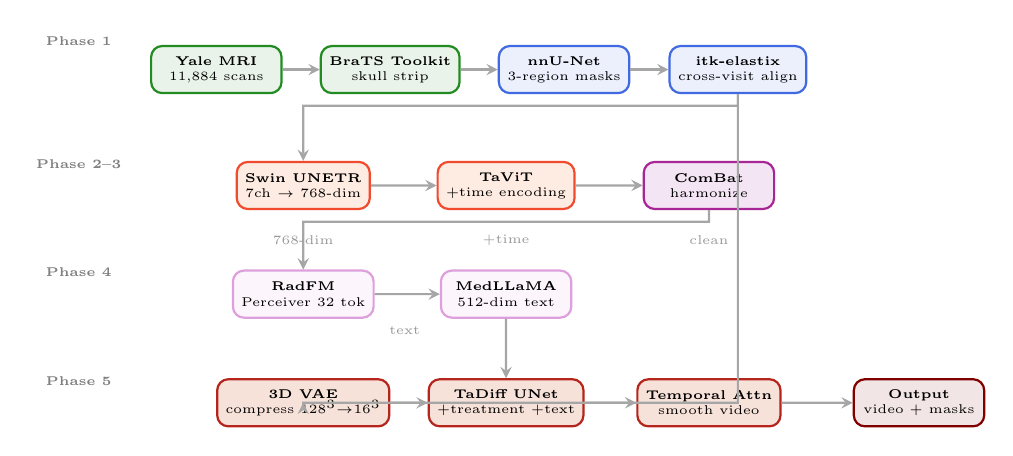
\begin{tikzpicture}[scale=0.92, every node/.style={transform shape},
            box/.style={rectangle, draw=#1, fill=#1!10, thick, minimum height=0.65cm, minimum width=1.8cm, align=center, rounded corners, font=\tiny},
            arr/.style={->, thick, >=stealth, color=gray!70},
            lbl/.style={font=\tiny\bfseries, color=gray},
            note/.style={font=\tiny, color=gray!80, align=center}
        ]

        % Phase 1
        \node[lbl] at (-2.4,0.4) {Phase 1};
        \node[box=ForestGreen] (raw) at (-0.5,0) {\textbf{Yale MRI}\\11,884 scans};
        \node[box=ForestGreen] (clean) at (1.9,0) {\textbf{BraTS Toolkit}\\skull strip};
        \node[box=RoyalBlue] (seg) at (4.3,0) {\textbf{nnU-Net}\\3-region masks};
        \node[box=RoyalBlue] (reg) at (6.7,0) {\textbf{itk-elastix}\\cross-visit align};

        \draw[arr] (raw) -- (clean);
        \draw[arr] (clean) -- (seg);
        \draw[arr] (seg) -- (reg);

        % Phase 2-3
        \node[lbl] at (-2.4,-1.3) {Phase 2--3};
        \node[box=RedOrange] (swin) at (0.7,-1.6) {\textbf{Swin UNETR}\\7ch $\to$ 768-dim};
        \node[box=RedOrange] (tavit) at (3.5,-1.6) {\textbf{TaViT}\\+time encoding};
        \node[box=Mulberry] (combat) at (6.3,-1.6) {\textbf{ComBat}\\harmonize};

        \draw[arr] (reg) -- ++(0,-0.5) -| (swin);
        \draw[arr] (swin) -- (tavit);
        \draw[arr] (tavit) -- (combat);

        % Phase 4
        \node[lbl] at (-2.4,-2.8) {Phase 4};
        \node[box=Plum] (radfm) at (0.7,-3.1) {\textbf{RadFM}\\Perceiver 32 tok};
        \node[box=Plum] (llm) at (3.5,-3.1) {\textbf{MedLLaMA}\\512-dim text};

        \draw[arr] (combat) -- ++(0,-0.5) -| (radfm);
        \draw[arr] (radfm) -- (llm);

        % Phase 5
        \node[lbl] at (-2.4,-4.3) {Phase 5};
        \node[box=BrickRed] (vae) at (0.7,-4.6) {\textbf{3D VAE}\\compress $128^3{\to}16^3$};
        \node[box=BrickRed] (tadiff) at (3.5,-4.6) {\textbf{TaDiff UNet}\\+treatment +text};
        \node[box=BrickRed] (temp) at (6.3,-4.6) {\textbf{Temporal Attn}\\smooth video};
        \node[box=Maroon] (out) at (9.2,-4.6) {\textbf{Output}\\video + masks};

        \draw[arr] (llm) -- ++(0,-0.5) -| (tadiff);
        \draw[arr] (reg) -- ++(0,-4.6) -| (vae);
        \draw[arr] (vae) -- (tadiff);
        \draw[arr] (tadiff) -- (temp);
        \draw[arr] (temp) -- (out);

        % Labels for what flows
        \node[note] at (0.7,-2.35) {768-dim};
        \node[note] at (3.5,-2.35) {+time};
        \node[note] at (6.3,-2.35) {clean};
        \node[note] at (2.1,-3.6) {text};

        \end{tikzpicture}
    \end{center}

    \vspace{0.1em}

    \begin{columns}
        \begin{column}{0.30\textwidth}
            \centering
            \scriptsize
            \textbf{Input per scan:}\\
            4 MRI + 3 masks = 7ch
        \end{column}
        \begin{column}{0.35\textwidth}
            \centering
            \scriptsize
            \textbf{Conditioning:}\\
            past scans + treatment + text
        \end{column}
        \begin{column}{0.30\textwidth}
            \centering
            \scriptsize
            \textbf{Output:}\\
            video + 3-region masks + uncertainty
        \end{column}
    \end{columns}
\end{frame}


% ============================================================================
% SLIDE 29: References
% ============================================================================
\begin{frame}[allowframebreaks]{Key References}
    \scriptsize
    \begin{thebibliography}{99}
        \bibitem{yale} Ramakrishnan et al., ``\href{https://doi.org/10.1038/s41597-025-04360-7}{Yale Brain Metastases Dataset},'' \textit{Scientific Data}, 2025
        \bibitem{cyprus} Trimithiotis et al., ``Cyprus PROTEAS Dataset,'' \textit{Zenodo}, 2025
        \bibitem{brats} Kofler et al., ``\href{https://doi.org/10.3389/fnins.2020.00125}{BraTS Toolkit},'' \textit{Frontiers in Neuroscience}, 2020
        \bibitem{nnunet} Isensee et al., ``\href{https://doi.org/10.1038/s41592-020-01008-z}{nnU-Net},'' \textit{Nature Methods}, 2021
        \bibitem{elastix} Niessen et al., ``\href{https://doi.org/10.21105/joss.05421}{itk-elastix},'' \textit{JOSS}, 2023
        \bibitem{gencombat} Horng et al., ``\href{https://doi.org/10.1038/s41598-022-08412-9}{Generalized ComBat},'' \textit{Scientific Reports}, 2022
        \bibitem{longcombat} Beer et al., ``\href{https://doi.org/10.1016/j.neuroimage.2020.117129}{Longitudinal ComBat},'' \textit{NeuroImage}, 2020
        \bibitem{combat} Fortin et al., ``\href{https://doi.org/10.2967/jnumed.121.262464}{ComBat Guide},'' \textit{J.\ Nuclear Medicine}, 2022
        \bibitem{swinunetr} Tang et al., ``\href{https://arxiv.org/abs/2201.01266}{Swin UNETR},'' CVPR 2022
        \bibitem{tavit} Hager et al., ``\href{https://arxiv.org/abs/2207.01032}{TaViT},'' 2022
        \bibitem{radfm} Wu et al., ``\href{https://arxiv.org/abs/2308.02463}{RadFM},'' 2025
        \bibitem{mmembed} Lin et al., ``MM-Embed,'' 2025
        \bibitem{ldm} Rombach et al., ``\href{https://arxiv.org/abs/2112.10752}{Latent Diffusion},'' CVPR 2022
        \bibitem{tadiff} Liu et al., ``\href{https://arxiv.org/abs/2309.05406}{Treatment-aware Diffusion},'' IEEE TMI 2025
        \bibitem{echonet} Reynaud et al., ``\href{https://arxiv.org/abs/2309.00997}{EchoNet-Synthetic},'' 2024
    \end{thebibliography}
\end{frame}

\end{document}
